\begin{figure}[htbp]
\centering
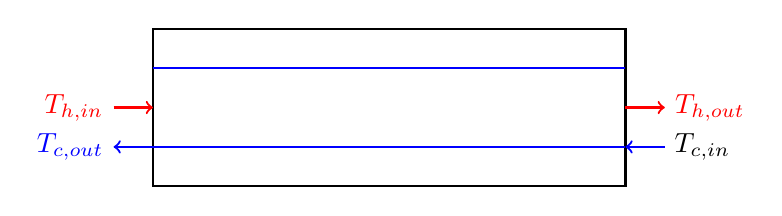
\begin{tikzpicture}
    % Shell
    \draw[thick] (0,0) rectangle (6,2);

    % Tubes (simplified)
    \draw[thick, blue] (0,0.5) -- (6,0.5);
    \draw[thick, blue] (0,1.5) -- (6,1.5);

    % Hot fluid
    \draw[->, thick, red] (-0.5,1) -- (0,1) node[left, pos=0] {$T_{h,\text{in}}$};
    \draw[->, thick, red] (6,1) -- (6.5,1) node[right] {$T_{h,\text{out}}$};

    % Cold fluid
    \draw[->, thick, blue] (6.5,0.5) -- (6,0.5);
    \draw[->, thick, blue] (0,0.5) -- (-0.5,0.5) node[left] {$T_{c,\text{out}}$};
    \node[right] at (6.5,0.5) {$T_{c,\text{in}}$};
\end{tikzpicture}
\caption{Counter-flow heat exchanger.}
\label{fig:heat_exchanger}
\end{figure}
